% Compilar con: pdflatex proyecto.tex  (dos veces para los enlaces/numeración)
\documentclass[12pt,letterpaper]{article}
\usepackage[utf8]{inputenc}
\usepackage[T1]{fontenc}
\usepackage[spanish,es-noshorthands]{babel}
\usepackage{mathptmx}                 % Times
\usepackage[margin=2.54cm]{geometry}
\usepackage{graphicx}
\usepackage{setspace}
\usepackage{microtype}
\usepackage{longtable,booktabs,array,calc}
\usepackage{enumitem}
\usepackage{xcolor}
\usepackage{listings}
\usepackage[hyphens]{url}
\usepackage[colorlinks=true,linkcolor=black,urlcolor=black,citecolor=black]{hyperref}
\usepackage{titlesec}
\usepackage{caption}
\usepackage{placeins}
\usepackage{float}
\usepackage{etoolbox}

% Columnas con ancho total acotado, incluido el espacio entre columnas.
\newcolumntype{L}[1]{>{\raggedright\arraybackslash}p{\dimexpr#1\linewidth-2\tabcolsep\relax}}
\newcolumntype{R}[1]{>{\raggedleft\arraybackslash}p{\dimexpr#1\linewidth-2\tabcolsep\relax}}
\newcolumntype{C}[1]{>{\centering\arraybackslash}p{\dimexpr#1\linewidth-2\tabcolsep\relax}}
\setlength{\tabcolsep}{5pt}
\setlength{\LTleft}{\fill}
\setlength{\LTright}{\fill}
\setlength{\LTpre}{10pt}
\setlength{\LTpost}{10pt}
\AtBeginEnvironment{longtable}{\small\setstretch{1.08}}
\captionsetup{font=small,labelfont=bf,labelsep=period,
  justification=justified,singlelinecheck=false,skip=8pt}
\captionsetup[longtable]{width=\textwidth}
\captionsetup[figure]{font={normalsize,stretch=1.08},skip=10pt}
\setlength{\emergencystretch}{2em}
\setlength{\textfloatsep}{16pt plus 3pt minus 3pt}
\setlength{\intextsep}{14pt plus 3pt minus 3pt}
\renewcommand{\topfraction}{0.9}
\renewcommand{\bottomfraction}{0.8}
\renewcommand{\textfraction}{0.08}
\renewcommand{\floatpagefraction}{0.7}
\setcounter{topnumber}{2}
\setcounter{bottomnumber}{2}
\setcounter{totalnumber}{3}
% Evita que las figuras pasen a una subsección posterior.
\pretocmd{\subsection}{\FloatBarrier}{}{}
\pretocmd{\subsubsection}{\FloatBarrier}{}{}

\setcounter{secnumdepth}{0}           % los números ya van en los títulos
\setstretch{1.15}
\setlength{\parindent}{0pt}
\setlength{\parskip}{6pt}
\titleformat{\section}{\normalfont\bfseries\fontsize{14}{16}\selectfont}{}{0pt}{}
\titleformat{\subsection}{\normalfont\bfseries\large}{}{0pt}{}
\providecommand{\tightlist}{\setlength{\itemsep}{2pt}\setlength{\parskip}{0pt}}
\renewcommand{\arraystretch}{1.2}
\urlstyle{same}
\Urlmuskip=0mu plus 1mu

\lstset{
  basicstyle=\ttfamily\footnotesize, breaklines=true, columns=fullflexible,
  frame=single, backgroundcolor=\color{black!4}, rulecolor=\color{black!30},
  keywordstyle=\bfseries, showstringspaces=false, inputencoding=utf8,
  extendedchars=true,
  literate={á}{{\'a}}1 {é}{{\'e}}1 {í}{{\'i}}1 {ó}{{\'o}}1 {ú}{{\'u}}1 {ñ}{{\~n}}1
}

\title{An\'alisis de patrones de siniestralidad vial en corredores principales de Bogot\'a mediante miner\'ia de datos}
\date{}
\hypersetup{pdftitle={Análisis de patrones de siniestralidad vial en corredores principales de Bogotá mediante minería de datos}}

\begin{document}

% ---------------- PORTADA ----------------
\begin{titlepage}
\centering
\setstretch{1.0}
\vspace*{0.2cm}
\IfFileExists{escudo.png}{%
  
\includegraphics[width=5.2cm,height=4.5cm,keepaspectratio]{escudo.png}\par
}{\vspace*{4.5cm}}

\vspace{0.8cm}
\begin{minipage}{0.94\textwidth}
\centering
{\bfseries\fontsize{18}{23}\selectfont
Análisis de patrones de siniestralidad vial en corredores principales de Bogotá mediante minería de datos\par}
\end{minipage}

\vspace{0.45cm}
{\fontsize{11}{14}\selectfont Entrega integrada del proyecto\par}
\vspace{0.8cm}
{\bfseries Metodología de la Investigación\par}

\vfill
\begin{minipage}{0.84\textwidth}
\centering
{\bfseries Integrantes\par}
\vspace{0.3cm}
\begingroup
\renewcommand{\arraystretch}{1.35}
\begin{tabular}{@{}l@{\hspace{0.8cm}}r@{}}
Gámez Camilo Andrés & 20231020193\\
Martínez Silva Gabriela & 20231020205\\
Velasco Rodríguez Carol Stefanya & 20231020215\\
Molina Diaz Kaleth & 20232020096
\end{tabular}\par
\endgroup
\end{minipage}

\vspace{0.8cm}
{\bfseries Docente\par}
\vspace{0.15cm}
Acosta Rodríguez Rafael Antonio\par

\vfill
{\bfseries Universidad Distrital Francisco José de Caldas\par}
\vspace{0.15cm}
Facultad de Ingeniería\par
Ingeniería de Sistemas\par
\vspace{0.5cm}
Bogotá D.C., 22 de octubre de 2026\par
\vspace*{0.2cm}
\end{titlepage}

% ---------------- TÍTULO ----------------
\begin{center}
{\bfseries\large Análisis de patrones de siniestralidad vial en corredores principales de Bogotá mediante minería de datos}
\end{center}

\textbf{Tema:} Prevención y análisis de accidentes de tránsito mediante minería de datos.

\hypertarget{introducciuxf3n}{%
\section{Introducción}\label{introducciuxf3n}}

La siniestralidad vial es un problema de seguridad, salud pública y
movilidad urbana: los accidentes de tránsito generan pérdidas humanas,
lesiones, daños materiales, congestión y costos sociales. En las grandes
ciudades los siniestros no se distribuyen de manera uniforme; algunos
corredores, intersecciones y tramos concentran más eventos, y ciertos
horarios, días y tipos de actor vial muestran comportamientos
recurrentes.

Bogotá no es la excepción. El Anuario de Siniestralidad Vial 2024
reportó más de 12 mil siniestros viales y 565 víctimas fatales. Los
motociclistas representaron el 47,3 \% de las personas fallecidas, los
sábados y viernes concentraron la mayor proporción de muertes (18,8 \% y
18,1 \%), la franja de mayor registro fue entre las 10:00 p.~m. y las
11:00 p.~m., y Kennedy, Engativá y Suba estuvieron entre las localidades
con más víctimas fatales. Estas cifras muestran que el problema tiene
una distribución territorial, temporal y poblacional diferenciada.

Cada siniestro queda documentado en el Informe Policial de Accidente de
Tránsito (IPAT), que registra lugar, fecha, hora, vehículos, actores
involucrados, circunstancias y condiciones de la vía. Estos registros se
publican en la base de siniestros viales del Sistema Integrado de
Información sobre Movilidad Urbana Regional (SIMUR). La ciudad ya
dispone de tableros que cuentan siniestros y víctimas, pero un conteo no
dice si una concentración es mayor de lo esperable ni qué condiciones
tienden a presentarse juntas. La riqueza de atributos del IPAT permite
ir más allá y preguntar dónde, cuándo, con quiénes y bajo qué
combinaciones de condiciones se repiten los siniestros.

Este proyecto estudia los siniestros ocurridos en 2024 en los diez
corredores principales de Bogotá con mayor número de registros.
Combina la estadística, para describir su distribución y contrastar
hipótesis sobre ella, con la minería de datos, para descubrir perfiles y
combinaciones frecuentes de características. Su propósito es describir y
explicar patrones en los registros existentes, no predecir accidentes
futuros ni establecer causas, de modo que los resultados sirvan para
priorizar corredores, horarios y actores viales en la prevención. La
pregunta que orienta el trabajo es:

\begin{quote}
{\fontfamily{lmr}\selectfont\textquestiondown}Qué patrones espaciales, temporales y de actor vial presentan los
siniestros viales ocurridos en 2024 en los principales corredores de
Bogotá, cuáles de ellos son estadísticamente significativos y cómo
pueden identificarse mediante técnicas de minería de datos?
\end{quote}

Para responderla, el documento revisa primero lo que se sabe sobre el
tema en el estado del arte, de donde surgen las hipótesis. Luego plantea los
objetivos, describe en la metodología cómo se contrastarán las hipótesis
y con qué datos, y finalmente presenta en el desarrollo el avance de la
ejecución.

\clearpage
\hypertarget{estado-del-arte}{%
\section{Estado del arte}\label{estado-del-arte}}

Esta sección revisa qué se conoce sobre la siniestralidad vial en
corredores urbanos, su distribución en el espacio y en el tiempo, los
actores más expuestos y el uso de la minería de datos para estudiarla.
Al final se sintetizan los vacíos que este proyecto aborda.

\hypertarget{siniestralidad-vial-como-fenuxf3meno-urbano}{%
\subsection{1. Siniestralidad vial como fenómeno
urbano}\label{siniestralidad-vial-como-fenuxf3meno-urbano}}

Los accidentes de tránsito son eventos multicausales. Chand, Jayesh y
Bhasi (2021) señalan que su estudio requiere considerar fuentes de
información y factores diversos: actores viales, vehículos,
infraestructura, entorno y tiempo de ocurrencia. Un siniestro no es un
hecho aislado: la repetición de eventos en un mismo tipo de vía, a
determinada hora o con actores específicos puede revelar patrones útiles
para la prevención.

En entornos urbanos influyen la intensidad de la movilidad, la
coexistencia de actores, la densidad de intersecciones, la velocidad, la
señalización, la iluminación y la configuración de la vía. Por eso los
corredores principales son especialmente relevantes: concentran grandes
flujos de automóviles, motocicletas, transporte público, ciclistas y
peatones, con interacciones más frecuentes y complejas. Vargas Montero
(2022) muestra, además, que los datos abiertos de accidentalidad de
Bogotá son una base suficiente para analizar el fenómeno en la ciudad.

\hypertarget{patrones-espaciales-y-corredores-cruxedticos}{%
\subsection{2. Patrones espaciales y corredores
críticos}\label{patrones-espaciales-y-corredores-cruxedticos}}

La identificación de puntos críticos (\emph{hotspots}) es una de las
líneas más consolidadas del área. Klaylee, Iamtrakul y Sornlertlamvanich
(2022) identifican puntos críticos de accidentes de motociclistas
mediante análisis espacial con sistemas de información geográfica; la
georreferenciación y el mapeo permiten localizar zonas de concentración
y diferenciar niveles de riesgo. En una ciudad, un punto crítico no se
reduce a una intersección: puede ser un tramo de avenida, un acceso, un
retorno o el entorno de una estación de transporte. Esto es relevante
en Bogotá, donde un mismo corredor atraviesa localidades con dinámicas
muy distintas.

Zhang, Zhu, Li, Qiu y Xie (2023) analizan patrones espacio-temporales de
accidentes con clustering de densidad y redes bayesianas, y muestran que
los patrones varían según el lugar y el momento: un sitio que no destaca
en un conteo anual puede concentrar eventos en horas pico, fines de
semana o periodos específicos. Ambos trabajos sugieren que los
siniestros no se reparten entre los corredores en proporción a su
tamaño, sino que algunos concentran más eventos de los esperados.

\hypertarget{patrones-temporales-y-actores-viales}{%
\subsection{3. Patrones temporales y actores
viales}\label{patrones-temporales-y-actores-viales}}

Los accidentes varían por hora, día de la semana, mes y condiciones de
luz. Las cifras de Bogotá citadas en la introducción, con las noches de
viernes y sábado como los momentos de mayor mortalidad, indican que el
tiempo no solo influye en cuántos siniestros ocurren, sino también en
qué tan graves son.

Los actores viales también tienen exposiciones distintas.
Ospina-Mateus, Berrio García, Quintana Jiménez y Salas-Navarro (2022)
documentan un conjunto de datos de accidentes de motociclistas en
Bogotá, lo que confirma la relevancia de este actor, que además
concentra casi la mitad de las muertes en la ciudad. Aun así, el
análisis de corredores no debe limitarse a un único actor: peatones,
ciclistas, pasajeros, conductores de automóvil, transporte público y
carga deben considerarse según la información disponible. Combinar
variables temporales y de actor vial permite construir perfiles de
siniestralidad, por ejemplo, corredores con recurrencia de siniestros de
motociclistas en horario nocturno o zonas con atropellos concentrados en
jornadas laborales.

\hypertarget{mineruxeda-de-datos-aplicada-a-accidentes}{%
\subsection{4. Minería de datos aplicada a
accidentes}\label{mineruxeda-de-datos-aplicada-a-accidentes}}

La minería de datos permite encontrar grupos y relaciones que no son
evidentes en bases extensas. Sathiyanathan y Warnajith (2024) integran
K-means y reglas de asociación para analizar seguridad vial: primero
forman grupos de accidentes similares y luego buscan combinaciones
frecuentes dentro de cada grupo, lo que ayuda a separar perfiles antes
de buscar relaciones. Shahin et al.~(2021) aplican el mismo principio a
accidentes en intersecciones, donde se repiten combinaciones de
horario, flujo, tipo de vehículo, condición vial y modalidad de
accidente.

Una regla de asociación se expresa como «A y B se presentan
frecuentemente junto con C». En siniestralidad vial, A y B podrían ser
un corredor y una franja horaria, y C un tipo de actor o de siniestro.
Su utilidad depende de tres indicadores: el soporte (frecuencia de la
combinación en la base), la confianza (proporción de casos en que, dado
el antecedente, ocurre el consecuente) y el \emph{lift} (si la
asociación supera lo esperado por la frecuencia individual de los
elementos; un valor mayor que 1 indica una asociación superior a la
esperada). Una regla no demuestra que un factor cause el accidente;
solo indica que una combinación ocurre con frecuencia en los registros.

Culajay Sandoval (2025) ofrece un antecedente latinoamericano: en
Guatemala aplica Apriori y FP-Growth, K-means y modelos supervisados
sobre registros históricos, e identifica asociaciones entre hora, día y
mes con la necesidad de hospitalización. Bejar Gladkowski (2023), por su
parte, desarrolla un análisis predictivo de accidentes en Madrid. Ambos
muestran que estas técnicas pueden extenderse a la predicción, una
posibilidad que este proyecto deja como ampliación posterior.

\hypertarget{prevenciuxf3n-y-comunicaciuxf3n-de-hallazgos}{%
\subsection{5. Prevención y comunicación de
hallazgos}\label{prevenciuxf3n-y-comunicaciuxf3n-de-hallazgos}}

El análisis de patrones debe contribuir a la prevención, con cautela.
Job (2022) estudia evaluaciones de intervenciones con cámaras de
velocidad y plantea que sus resultados varían según el contexto, los
métodos de evaluación y las condiciones de implementación. Una
concentración de siniestros no demuestra, por sí sola, que una
intervención concreta sea la solución; las medidas que se deriven del
análisis deben presentarse como alternativas sujetas a validación
institucional.

La comunicación clara también importa. Ordoñez Cueto y Fernández Ebratt
(2025) desarrollan un tablero de accidentes para Barranquilla y muestran
que indicadores, mapas, gráficos y filtros facilitan el acceso a
información compleja. Bogotá ya cuenta con un tablero público de
siniestralidad por fecha, actor vial, localidad y corredor; el aporte de
este proyecto no es reemplazarlo, sino añadir la evidencia estadística y
los patrones que un conteo no muestra.

\hypertarget{suxedntesis-y-aporte-del-proyecto}{%
\subsection{6. Síntesis y aporte del
proyecto}\label{suxedntesis-y-aporte-del-proyecto}}

La literatura coincide en que la siniestralidad vial urbana no es
aleatoria ni homogénea, y deja tres ideas que este proyecto convierte en
hipótesis verificables para los corredores de Bogotá: que algunos
corredores concentran más siniestros de los que corresponderían a su
longitud (apartado de patrones espaciales); que la gravedad de los siniestros depende del
momento en que ocurren (apartado de patrones temporales y actores viales); y que los siniestros con
motocicleta tienen más víctimas que los demás (mismo apartado). A esto se
suma que la combinación de clustering y reglas de asociación (apartado de
minería de datos) permite describir perfiles y combinaciones que las cifras agregadas
no revelan.

El aporte del proyecto es, por tanto, doble: comprobar con pruebas
estadísticas si esos patrones se cumplen en los corredores principales
de Bogotá durante 2024, y describir con minería de datos los perfiles y
combinaciones que los acompañan. Los objetivos de la siguiente sección
se derivan directamente de esta síntesis.

\clearpage
\hypertarget{objetivos}{%
\section{Objetivos}\label{objetivos}}

\hypertarget{objetivo-general}{%
\subsection{1. Objetivo general}\label{objetivo-general}}

Determinar los patrones espaciales, temporales y de actor vial de los
siniestros ocurridos en 2024 en los diez corredores principales de
Bogotá con mayor número de registros, mediante pruebas de hipótesis
estadísticas y técnicas de minería de datos aplicadas a la base de
siniestros viales del SIMUR, con el fin de priorizar corredores, franjas
horarias y actores viales como insumo para la prevención.

\hypertarget{objetivos-especuxedficos}{%
\subsection{2. Objetivos específicos}\label{objetivos-especuxedficos}}

Cada objetivo específico enuncia primero la meta que se persigue y
luego el entregable, destacado en cursiva, con el que se da por
cumplido. Los objetivos siguen el orden del estudio: cada entregable es
el insumo del objetivo siguiente.

\begin{enumerate}[label=\textbf{\arabic*.}, leftmargin=*, align=left, itemsep=6pt]
\item
  Construir una base de datos depurada y documentada de los siniestros
  de 2024 en los diez corredores seleccionados. Se cumple con la entrega
  de \emph{un diccionario de variables, la lista de corredores con su
  longitud y una base limpia con al menos diez variables y menos del
  5 \% de valores nulos en las variables clave}, acompañada de la
  trazabilidad de los registros descartados.
\item
  Caracterizar la distribución espacial y temporal de los siniestros por
  corredor, mes, día de la semana, franja horaria y actor vial. Se
  cumple con la entrega de \emph{las tablas de frecuencias y tasas por
  kilómetro, al menos un mapa de concentración y cuatro gráficos}, que
  identifiquen los tres corredores y las tres franjas horarias de mayor
  concentración.
\item
  Contrastar las hipótesis sobre concentración espacial, franja horaria
  y actor vial con un nivel de significancia de 0,05. Se cumple con la
  entrega de \emph{una tabla de resultados que reporte, para cada
  hipótesis, el estadístico, el p-valor, el tamaño del efecto y la
  decisión}, junto con su interpretación.
\item
  Identificar perfiles de siniestralidad mediante algoritmos de
  agrupamiento (K-means y DBSCAN). Se cumple con la entrega de \emph{una
  ficha descriptiva para cada uno de los tres a ocho perfiles
  obtenidos}, con sus variables dominantes y su composición de
  gravedad.
\item
  Descubrir asociaciones frecuentes entre las características de los
  siniestros, de forma global y dentro de cada perfil. Se cumple con la
  entrega de \emph{al menos diez reglas de asociación interpretadas} que
  superen los umbrales mínimos de soporte, confianza y \emph{lift}.
\item
  Integrar y comunicar los resultados del estudio. Se cumple con la
  entrega de \emph{un tablero analítico con al menos cuatro vistas
  (mapa, comportamiento temporal, perfiles y reglas) y un informe final
  con al menos tres propuestas preventivas}.
\end{enumerate}

\clearpage
\hypertarget{metodologuxeda}{%
\section{Metodología}\label{metodologuxeda}}

\hypertarget{paradigma-y-enfoque}{%
\subsection{1. Paradigma y enfoque}\label{paradigma-y-enfoque}}

La investigación se ubica en el paradigma positivista, en su versión
pospositivista: asume que la siniestralidad vial puede observarse y
medirse de forma objetiva a partir de registros, y que las afirmaciones
sobre ella deben contrastarse con datos. En coherencia, el enfoque es
cuantitativo y el método es hipotético-deductivo: las ideas que deja el
estado del arte se formulan como hipótesis estadísticas y se aceptan o
rechazan con pruebas de significancia.

El estudio se aborda desde el lado estadístico. La estadística
descriptiva caracteriza la distribución de los siniestros mediante
frecuencias, proporciones y tasas por kilómetro, y la estadística
inferencial contrasta las hipótesis. La minería de datos complementa
este trabajo: descubre perfiles y combinaciones de características que
luego se interpretan a la luz de las pruebas. Se descarta un enfoque
cualitativo porque la pregunta busca patrones medibles en un volumen
grande de registros, no la experiencia o el significado que los actores
dan a los siniestros. Por la misma razón no se adopta un enfoque mixto:
la investigación no recoge datos cualitativos, como entrevistas u
observación, que deban integrarse con los cuantitativos.

\hypertarget{alcance-y-diseuxf1o}{%
\subsection{2. Alcance y diseño}\label{alcance-y-diseuxf1o}}

El alcance es descriptivo-correlacional: el estudio describe cómo se
distribuyen los siniestros y mide la asociación entre sus
características, sin establecer relaciones de causalidad. Tampoco busca
predecir siniestros futuros con redes neuronales u otros modelos
complejos. Solo si la variable de gravedad resulta completa y confiable
se evaluará, como componente complementario, un árbol de decisión o un
Random Forest para clasificarla.

El diseño es no experimental, transversal y retrospectivo: las variables
no se manipulan, sino que se analizan datos secundarios de hechos ya
ocurridos. Un diseño experimental o cuasiexperimental no es posible,
porque exigiría provocar siniestros o asignar corredores a condiciones
controladas, y tampoco es necesario, porque el estudio no evalúa el
efecto de una intervención.

La investigación se plantea como un estudio de caso único: el caso son
los corredores principales de Bogotá durante 2024. Esta estrategia
permite analizar a fondo un contexto concreto, con sus propios datos y
dinámicas, aunque sus conclusiones no se generalizan automáticamente a
otras ciudades o periodos.

\hypertarget{hipuxf3tesis}{%
\subsection{3. Hipótesis}\label{hipuxf3tesis}}

Las tres ideas de la síntesis del estado del arte se
formulan como hipótesis estadísticas, cada una con su prueba.

\textbf{H1. Concentración espacial.}
\begin{itemize}
\tightlist
\item
  $H_0$: el número de siniestros en cada corredor es proporcional a su
  longitud.
\item
  $H_1$: algunos corredores concentran más siniestros de los esperados
  por su longitud.
\item
  Prueba: chi-cuadrado de bondad de ajuste, con frecuencias esperadas
  proporcionales a la longitud de cada corredor.
\end{itemize}

\textbf{H2. Franja horaria y gravedad.}
\begin{itemize}
\tightlist
\item
  $H_0$: la gravedad del siniestro (solo daños, con heridos o con
  muertos) es independiente de la franja horaria y del tipo de día
  (entre semana o fin de semana).
\item
  $H_1$: la gravedad depende de la franja horaria y del tipo de día; las
  noches de fin de semana presentan mayor proporción de siniestros
  graves.
\item
  Prueba: chi-cuadrado de independencia, con V de Cramér como tamaño del
  efecto.
\end{itemize}

\textbf{H3. Actor vial y gravedad.}
\begin{itemize}
\tightlist
\item
  $H_0$: la proporción de siniestros con víctimas (heridos o muertos) es
  igual en los que involucran motocicleta y en los que no.
\item
  $H_1$: la proporción es mayor en los siniestros con motocicleta.
\item
  Prueba: prueba z unilateral de diferencia de proporciones y razón de
  momios con intervalo de confianza del 95 \%.
\end{itemize}

Se rechaza $H_0$ cuando el p-valor es menor que 0,05, con corrección de
Bonferroni por realizar varias pruebas. Como en una base grande casi
cualquier diferencia resulta significativa, cada resultado se interpreta
junto con su tamaño del efecto (V de Cramér: 0,1 pequeño, 0,3 mediano y
0,5 grande).

\hypertarget{poblaciuxf3n-y-muestra}{%
\subsection{4. Población y muestra}\label{poblaciuxf3n-y-muestra}}

Los datos provienen de la base de siniestros viales de Bogotá del SIMUR,
construida a partir del IPAT. La unidad de análisis es el siniestro
vial, es decir, cada registro de esa base; para H3 se consideran
también los actores viales asociados a cada siniestro.

La población objetivo son los siniestros viales ocurridos en los
corredores principales de Bogotá, y la población accesible, los
siniestros de 2024 registrados en la base del SIMUR en los diez
corredores con mayor número de registros ese año. Se incluyen los
registros con fecha y hora válidas, corredor identificable, coordenadas
dentro de Bogotá y gravedad registrada; se excluyen los duplicados y los
que tengan fechas, horas o coordenadas inválidas.

La selección se hace en dos etapas. En la primera, los corredores se
eligen mediante un muestreo no probabilístico por criterio: se toman los
diez con mayor número de siniestros en 2024, porque son los de mayor
interés para la prevención. En la segunda, dentro de esos corredores se
trabaja con un censo, es decir, con todos los siniestros que cumplen los
criterios de inclusión. La base completa está disponible sin costo, así
que tomar todos los datos posibles aprovecha toda la información y evita
el error de muestreo. El tamaño final ($N$) se reportará después de la
depuración.

\hypertarget{variables}{%
\subsection{5. Variables}\label{variables}}

La selección final de variables dependerá de la estructura y
completitud de la base. Las previstas, y su papel en las hipótesis, son:

\begingroup
\begin{longtable}{@{}L{0.18}L{0.38}L{0.19}L{0.25}@{}}
\toprule
\textbf{Dimensión} & \textbf{Variables} & \textbf{Tipo} & \textbf{Papel} \\
\midrule
\endfirsthead
\toprule
\textbf{Dimensión} & \textbf{Variables} & \textbf{Tipo} & \textbf{Papel} \\
\midrule
\endhead
Espacial & Corredor, localidad, tramo o intersección, coordenadas & Nominal & Independiente (H1) \\
 & Longitud del corredor (km) & Razón & Valor esperado (H1) \\
Temporal & Mes, día de la semana, fin de semana, hora y franja horaria & Ordinal y nominal & Independiente (H2) \\
Actor y vehículo & Actor vial, tipo de vehículo, motocicleta involucrada & Nominal y dicotómica & Independiente (H3) \\
Evento & Clase de siniestro & Nominal & Descriptiva \\
 & Gravedad (solo daños, con heridos, con muertos) & Ordinal & Dependiente (H2 y H3) \\
\bottomrule
\end{longtable}
\endgroup

\hypertarget{fases-del-estudio}{%
\subsection{6. Fases del estudio}\label{fases-del-estudio}}

\begin{enumerate}
\def\labelenumi{\arabic{enumi}.}
\tightlist
\item
  \textbf{Preparación de datos:} revisión de la estructura de la base,
  depuración de duplicados, nulos e inconsistencias de fecha, hora y
  coordenadas, estandarización de categorías y selección de los
  corredores.
\item
  \textbf{Análisis descriptivo:} frecuencias, proporciones y tasas por
  kilómetro por corredor, localidad, mes, día, franja horaria, actor
  vial y tipo de siniestro, con mapas de concentración elaborados con
  apoyo de SIG.
\item
  \textbf{Contraste de hipótesis:} aplicación de las pruebas descritas
  en el apartado de hipótesis, con verificación previa de supuestos (frecuencias
  esperadas de al menos 5) y cálculo del tamaño del efecto.
\item
  \textbf{Clustering:} agrupamiento de los siniestros con K-means sobre
  variables codificadas y con DBSCAN sobre coordenadas para detectar
  zonas densas. El número de grupos se elige con el coeficiente de
  silueta y el método del codo, y cada grupo se describe por sus
  variables dominantes; una prueba chi-cuadrado indica si su composición
  de gravedad difiere.
\item
  \textbf{Reglas de asociación:} transformación de los registros en
  transacciones (corredor, franja, día, actor vial, vehículo y tipo de
  siniestro) y aplicación de Apriori o FP-Growth, de forma global y por
  grupo, siguiendo la secuencia de Sathiyanathan y Warnajith (2024). Las
  reglas se filtran por soporte, confianza y \emph{lift}, con umbrales
  definidos tras observar la distribución de la base.
\item
  \textbf{Visualización e interpretación:} integración de mapas,
  indicadores por corredor, comportamiento temporal, resultados de las
  hipótesis, perfiles y reglas en un tablero analítico, y redacción del
  informe con las propuestas preventivas.
\end{enumerate}

\hypertarget{herramientas}{%
\subsection{7. Herramientas}\label{herramientas}}

El análisis se realizará en Python: pandas para la depuración, SciPy y
statsmodels para las pruebas de hipótesis, scikit-learn para K-means,
DBSCAN y el coeficiente de silueta, mlxtend para Apriori y FP-Growth,
geopandas y folium para el análisis espacial y los mapas, y Plotly o
Streamlit para el tablero.

\hypertarget{consideraciones-y-limitaciones}{%
\subsection{8. Consideraciones y
limitaciones}\label{consideraciones-y-limitaciones}}

La calidad de los resultados depende del subregistro y de la
completitud del IPAT, y, como corresponde a un estudio de caso, sus
conclusiones se limitan a los corredores seleccionados y al año 2024. Como se señaló en el estado del arte, las
recomendaciones preventivas se formularán como propuestas sujetas a
validación institucional y no como soluciones comprobadas.

\clearpage
\hypertarget{desarrollo}{%
\section{Desarrollo}\label{desarrollo}}

Esta sección presenta la ejecución y los resultados de los dos primeros
objetivos específicos: la construcción de la base depurada y documentada,
y la caracterización espacial, temporal y de actor vial. El desarrollo
sigue las cuatro primeras etapas de la metodología. Los contrastes de
hipótesis, los perfiles de agrupamiento, las reglas de asociación y las
propuestas preventivas corresponden a objetivos posteriores y no se
desarrollan en este apartado.

\hypertarget{plan-de-trabajo}{%
\subsection{1. Plan de trabajo}\label{plan-de-trabajo}}

Las actividades ejecutadas y sus productos se sintetizan en la tabla
\ref{tab:avance-oe12}. En las etapas 1 a 3 se cumplió el primer objetivo;
en la etapa 4 se elaboraron los entregables del segundo. Todos los
conteos que se presentan a continuación se obtuvieron con los módulos
\texttt{preparar} y \texttt{describir} del programa del proyecto.

\begingroup
\begin{longtable}{@{}C{0.11}L{0.35}C{0.10}L{0.44}@{}}
\caption{Actividades ejecutadas para los objetivos específicos 1 y 2.}\label{tab:avance-oe12}\\
\toprule
\textbf{Etapa} & \textbf{Actividad} & \textbf{OE} & \textbf{Producto obtenido}\\
\midrule
\endfirsthead
\toprule
\textbf{Etapa} & \textbf{Actividad} & \textbf{OE} & \textbf{Producto obtenido}\\
\midrule
\endhead
1 & Revisar la estructura y documentar las variables & 1 & Perfil de los 40 campos originales y definición de variables de análisis\\
2 & Normalizar direcciones y seleccionar corredores & 1 & Diez corredores identificados, con su longitud\\
3 & Depurar y estandarizar los registros & 1 & Base de 3.624 siniestros, trazabilidad y control de nulos\\
4 & Caracterizar la distribución espacio-temporal y los actores & 2 & Nueve tablas, seis gráficos, un mapa estático y un mapa interactivo\\
\bottomrule
\end{longtable}
\endgroup

\hypertarget{etapa-1-adquisiciuxf3n-y-diccionario-de-variables}{%
\subsection{2. Revisión de la base y diccionario de variables}\label{etapa-1-adquisiciuxf3n-y-diccionario-de-variables}}

Se utilizó el archivo \texttt{datos.zip}, suministrado al equipo como
exportación en CSV de la base del SIMUR. Contiene los archivos de
siniestros, vehículos, actores y diccionario. La unidad de análisis se
mantuvo en el siniestro: las caracterizaciones de los dos primeros
objetivos se calcularon sobre la tabla de siniestros, sin unir las tablas
de vehículos y personas, para evitar multiplicar un evento por el número
de participantes.

La lectura identificó 278.614 registros y 40 columnas originales. Aunque
el recurso se identifica con el anuario de 2024, el archivo recibido
incluye registros de otros años; por ello no se trató su totalidad como
población de 2024. La delimitación temporal dejó 13.949 siniestros de ese
año para la selección de corredores. La base final cubre del 1 de enero
al 31 de diciembre de 2024.

Se generó un perfil de cada campo con su nombre, tipo de lectura,
número y porcentaje de nulos, valores distintos y ejemplos. Los campos
se leyeron inicialmente como texto para conservar identificadores y
homogeneizar las conversiones. Por ejemplo, las coordenadas presentaban
coma decimal y se convirtieron a valores numéricos. El perfil completo
quedó en \texttt{diccionario\_variables.csv}; su columna de descripción
no está diligenciada por el generador automático, por lo que la tabla
\ref{tab:diccionario-oe1} explicita el significado operativo de las
principales variables utilizadas.

\begingroup
\begin{longtable}{@{}L{0.25}L{0.18}L{0.57}@{}}
\caption{Diccionario operativo de las variables principales de la base de análisis.}\label{tab:diccionario-oe1}\\
\toprule
\textbf{Variable} & \textbf{Tipo final} & \textbf{Definición y tratamiento}\\
\midrule
\endfirsthead
\toprule
\textbf{Variable} & \textbf{Tipo final} & \textbf{Definición y tratamiento}\\
\midrule
\endhead
Código del accidente & Identificador & Campo original que identifica el siniestro y permite controlar duplicados.\\
Fecha & Fecha & Fecha de ocurrencia convertida a formato de fecha; delimita el año de estudio.\\
Hora & Entero, 0--23 & Hora de ocurrencia; se conserva además el minuto original, pero las agrupaciones se hacen por hora.\\
Latitud y longitud & Numérico & Coordenadas del registro, utilizadas para validar ubicación y elaborar los mapas.\\
Localidad & Categórico & Localidad declarada en el registro; se normalizó su escritura, sin reasignarla mediante límites cartográficos.\\
Vía principal y vía que cruza & Categórico & Ejes extraídos de la dirección y normalizados a una nomenclatura común.\\
Corredor & Categórico & Uno de los diez ejes seleccionados; cada siniestro recibe una sola asignación.\\
Gravedad & Ordinal & Solo daños, con heridos o con muertos, a partir del indicador tradicional.\\
Clase & Categórico & Modalidad del evento: choque, atropello, caída de ocupante, volcamiento, otro o incendio en la base final.\\
Mes & Entero, 1--12 & Mes derivado de la fecha de ocurrencia.\\
Día de la semana & Categórico ordenado & De lunes a domingo, derivado de la fecha.\\
Fin de semana & Booleano & Verdadero para sábado o domingo; no incorpora los festivos entre semana.\\
Franja horaria & Categórico ordenado & Madrugada [0,6), mañana [6,10), mediodía [10,16), tarde [16,20) y noche [20,24).\\
Motocicleta involucrada & Booleano & Presencia de la marca afirmativa en el indicador de motocicleta.\\
Otros indicadores de participación & Booleano & Presencia registrada de peatón, bicicleta, carga, transporte público, persona mayor o menor de edad, entre otros.\\
Con víctimas & Booleano & Verdadero si la gravedad corresponde a heridos o muertos; no representa un conteo de personas.\\
\bottomrule
\end{longtable}
\endgroup

El perfil de la base cruda mostró un 5,41\,\% de nulos en las
coordenadas y un 96,23\,\% en el tipo de objeto fijo. Estos porcentajes
corresponden al archivo multianual, no a la base final. Además, algunos
campos solo aplican a determinados eventos: no se interpretó la ausencia
de tipo de objeto fijo como una falla general del registro.

Los indicadores \texttt{Con\_*} presentan una marca \texttt{SI} cuando
se registra la característica. El programa transforma las celdas vacías
en falso, entendido como ausencia de marca afirmativa. Esta regla permite
calcular participaciones, pero no verifica por sí misma la ausencia real
del actor o la condición. Por tanto, la completitud de los indicadores
transformados debe interpretarse junto con esa decisión de codificación.
Para la gravedad se utilizó el indicador tradicional, sin mezclarlo con
el indicador de seguimiento a 30 días.

\hypertarget{etapa-2-definiciuxf3n-de-corredores-y-periodo}{%
\subsection{3. Selección de corredores}\label{etapa-2-definiciuxf3n-de-corredores-y-periodo}}

La base no contiene una variable de corredor. Se construyó a partir de
la dirección, unificando abreviaturas de calles y carreras y equivalencias
de avenidas: por ejemplo, Avenida Boyacá se identificó como Carrera 72.
Se reconocieron tanto la vía principal como la vía que cruza. Sobre los
13.949 registros válidos de 2024 se seleccionaron los diez ejes con más
apariciones, sin realizar una selección aleatoria.

\begingroup
\begin{longtable}{@{}C{0.10}L{0.48}R{0.20}R{0.22}@{}}
\caption{Corredores seleccionados por apariciones en las direcciones de 2024.}\label{tab:seleccion-corredores}\\
\toprule
\textbf{Orden} & \textbf{Corredor} & \textbf{Apariciones} & \textbf{Longitud}\newline\textbf{(km)}\\
\midrule
\endfirsthead
\toprule
\textbf{Orden} & \textbf{Corredor} & \textbf{Apariciones} & \textbf{Longitud}\newline\textbf{(km)}\\
\midrule
\endhead
1 & Avenida Boyacá & 637 & 52,1\\
2 & Avenida Caracas & 525 & 25,0\\
3 & Avenida Ciudad de Cali & 470 & 23,6\\
4 & Avenida NQS (Carrera 30) & 467 & 17,5\\
5 & Carrera Séptima & 316 & 24,7\\
6 & Avenida Carrera 10 & 297 & 7,6\\
7 & Avenida El Dorado (Calle 26) & 288 & 22,6\\
8 & Avenida Calle 6 & 274 & 8,9\\
9 & Autopista Norte & 267 & 28,4\\
10 & Avenida Centenario (Calle 13) & 259 & 16,2\\
\bottomrule
\end{longtable}
\endgroup

La selección y el conteo final responden a reglas distintas. Para elegir
los corredores, un cruce puede aportar una aparición a cada uno de sus
dos ejes. Después, si ambas vías están entre las seleccionadas, el
siniestro se asigna a la vía principal; si solo está seleccionada la vía
que cruza, se asigna a esta. Así se evita contar dos veces un mismo
siniestro en los resultados descriptivos. Por esta razón, las apariciones
de la tabla \ref{tab:seleccion-corredores} no deben sumarse como eventos
únicos ni confundirse con las frecuencias de la tabla
\ref{tab:distribucion-corredores}.

Las longitudes se incorporaron del archivo de insumos externos del
proyecto. Este registra OpenStreetMap como fuente para nueve corredores
y Wikipedia para la Avenida Caracas, e incluye notas sobre los tramos
considerados en Boyacá, Ciudad de Cali y Centenario. Se emplearon como
longitudes de referencia: no se realizó una nueva medición cartográfica
ni una homologación de sus límites en esta etapa. Las tasas por kilómetro
son sensibles a esa delimitación y no sustituyen una medida de exposición
basada en flujos de tránsito.

\hypertarget{etapa-3-depuraciuxf3n-y-estandarizaciuxf3n}{%
\subsection{4. Depuración y estandarización}\label{etapa-3-depuraciuxf3n-y-estandarizaciuxf3n}}

La depuración se ejecutó de forma secuencial y conservó los campos
originales junto con las variables tipadas y derivadas. Se controlaron
los duplicados por código de accidente, las fechas y horas inválidas, la
ubicación y la gravedad. Para las coordenadas se utilizó la ventana
geográfica definida en el programa: latitud entre 3,70 y 4,85 y longitud
entre $-74,45$ y $-73,95$. Este filtro comprueba plausibilidad regional;
no equivale a validar pertenencia al polígono oficial de Bogotá ni a
comprobar que el punto esté sobre el corredor asignado.

\begingroup
\begin{longtable}{@{}L{0.62}R{0.19}R{0.19}@{}}
\caption{Trazabilidad de la construcción de la base de análisis.}\label{tab:trazabilidad}\\
\toprule
\textbf{Paso} & \textbf{Descartados} & \textbf{Conservados}\\
\midrule
\endfirsthead
\toprule
\textbf{Paso} & \textbf{Descartados} & \textbf{Conservados}\\
\midrule
\endhead
Archivo original & --- & 278.614\\
Duplicados por código & 0 & 278.614\\
Fecha inválida & 0 & 278.614\\
Registros fuera de 2024 & 264.665 & 13.949\\
Hora inválida & 0 & 13.949\\
Coordenadas fuera de la ventana de validación & 0 & 13.949\\
Gravedad sin registrar & 0 & 13.949\\
Dirección sin vía identificable & 0 & 13.949\\
Fuera de los diez corredores seleccionados & 10.325 & 3.624\\
\bottomrule
\end{longtable}
\endgroup

La reducción principal correspondió a la delimitación temporal, no a la
eliminación de registros de mala calidad. Dentro del subconjunto de 2024
no se descartaron eventos por hora, coordenadas, gravedad o dirección
bajo las reglas implementadas. Los 3.624 siniestros retenidos representan
el 25,98\,\% de los 13.949 registros de 2024; los restantes quedaron fuera
por no pertenecer a los diez ejes seleccionados.

Se derivaron el mes, el día, el fin de semana, la franja horaria y el
indicador de víctimas. Las franjas son intervalos cerrados a la izquierda
y abiertos a la derecha: un evento a las 06:00 pertenece a la mañana y
uno a las 20:00 a la noche. Los nombres de localidad y clase se
normalizaron para evitar categorías separadas por tildes o diferencias
de escritura.

La base final contiene 77 columnas, incluidas las 40 originales. En
corredor, fecha, hora, gravedad y motocicleta involucrada se obtuvo un
0\,\% de nulos, por debajo del umbral del 5\,\% fijado en el primer
objetivo. En el indicador de motocicleta, este resultado depende de la
codificación de celdas vacías descrita anteriormente; no debe confundirse
con una validación independiente de la calidad del reporte.

Como entregables quedaron la base limpia en formato Parquet, el perfil
de variables, la lista de corredores con longitudes, la trazabilidad y
el informe de nulos. Con ello se dispone de una base con más de diez
variables y controles explícitos para continuar el análisis. La
reproducción de esta etapa se realiza desde la raíz del repositorio:

\begin{lstlisting}[language=bash]
python -m siniestralidad.preparar
python -m siniestralidad.describir
\end{lstlisting}

\hypertarget{analisis-descriptivo-oe2}{%
\subsection{5. Análisis descriptivo espacial, temporal y de actor vial}\label{analisis-descriptivo-oe2}}

El segundo objetivo se desarrolló sobre los 3.624 eventos únicos de la
base depurada. Se calcularon frecuencias absolutas y relativas por
corredor, localidad, mes, día, franja, clase y gravedad, además de las
participaciones por actor y vehículo y la matriz de día por hora. Los
porcentajes generales utilizan como denominador los 3.624 siniestros,
salvo cuando se indica expresamente una composición dentro de cada
franja. Los resultados describen registros observados: no prueban
asociaciones estadísticas ni relaciones causales.

\subsubsection{5.1. Distribución por corredor y concentración espacial}

\begingroup
\begin{longtable}{@{}L{0.43}R{0.15}R{0.13}R{0.12}R{0.17}@{}}
\caption{Distribución de eventos únicos y tasa descriptiva por kilómetro.}\label{tab:distribucion-corredores}\\
\toprule
\textbf{Corredor} & \textbf{Eventos} & \textbf{\%} & \textbf{km} & \textbf{Por km}\\
\midrule
\endfirsthead
\toprule
\textbf{Corredor} & \textbf{Eventos} & \textbf{\%} & \textbf{km} & \textbf{Por km}\\
\midrule
\endhead
Avenida Boyacá & 619 & 17,08 & 52,1 & 11,88\\
Avenida Caracas & 513 & 14,16 & 25,0 & 20,52\\
Avenida NQS (Carrera 30) & 458 & 12,64 & 17,5 & 26,17\\
Avenida Ciudad de Cali & 455 & 12,56 & 23,6 & 19,28\\
Carrera Séptima & 313 & 8,64 & 24,7 & 12,67\\
Avenida Carrera 10 & 285 & 7,86 & 7,6 & 37,50\\
Autopista Norte & 266 & 7,34 & 28,4 & 9,37\\
Avenida El Dorado (Calle 26) & 246 & 6,79 & 22,6 & 10,88\\
Avenida Centenario (Calle 13) & 239 & 6,59 & 16,2 & 14,75\\
Avenida Calle 6 & 230 & 6,35 & 8,9 & 25,84\\
\midrule
Total & 3.624 & 100,00 & & \\
\bottomrule
\end{longtable}
\endgroup

Por número de siniestros asignados, los tres primeros corredores fueron
Boyacá, Caracas y NQS: sumaron 1.590 eventos, el 43,87\,\% de la base.
NQS pasó por encima de Ciudad de Cali al aplicar la asignación única,
aunque Ciudad de Cali había registrado más apariciones durante la
selección. Esto muestra la importancia de mantener explícita la regla
de conteo.

La tasa descriptiva se calculó como $T_c=n_c/L_c$, donde $n_c$ es el
número anual de eventos asignados al corredor y $L_c$ su longitud de
referencia en kilómetros. Al ajustar por longitud, los tres mayores
valores correspondieron a Carrera 10 (37,50), NQS (26,17) y Calle 6
(25,84), como muestra la figura \ref{fig:oe2-corredores}. Boyacá lideró
el volumen absoluto, pero su mayor longitud hizo que no liderara este
indicador. Se trata de concentración de registros por unidad de longitud;
sin aforos de vehículos o personas no puede interpretarse como
probabilidad individual de sufrir un siniestro.

% Bloque indivisible: la imagen y su pie pasan juntos a la página siguiente.
\begin{figure}[H]
\begin{minipage}{\linewidth}
\centering
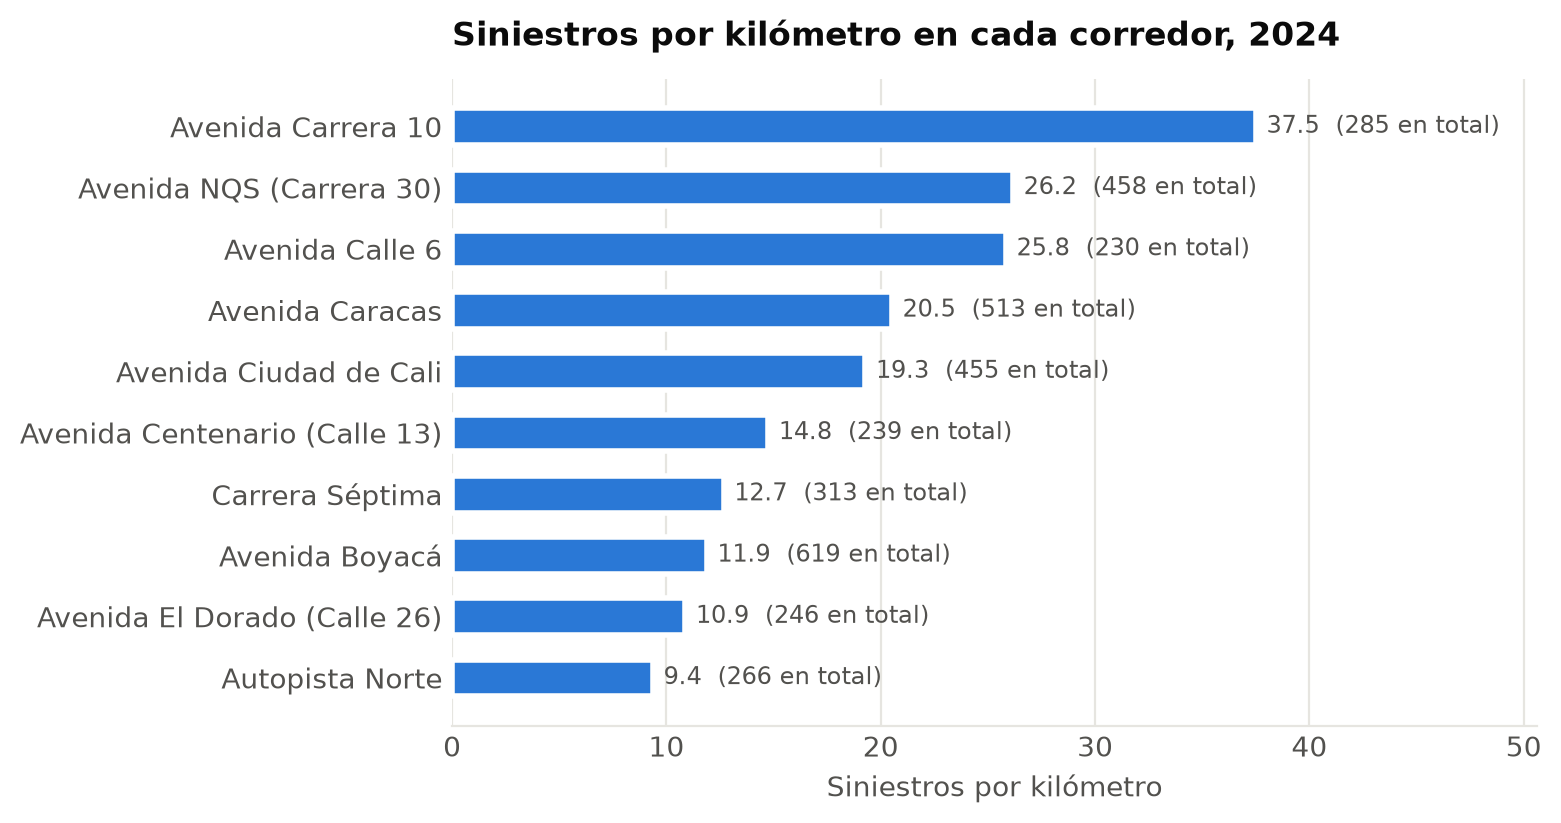
\includegraphics[width=\linewidth,height=0.40\textheight,keepaspectratio]{figuras/oe2_corredores_por_km.png}
\caption{Siniestros por kilómetro en los corredores seleccionados. Entre paréntesis se muestra el conteo de eventos únicos. Fuente: elaboración propia con la base depurada y las longitudes del proyecto.}
\label{fig:oe2-corredores}
\end{minipage}
\end{figure}

Por localidad declarada, Kennedy registró 486 eventos (13,41\,\%),
Usaquén 361 (9,96\,\%) y Fontibón 350 (9,66\,\%). Estos resultados
corresponden exclusivamente a los corredores seleccionados, no al total
de siniestros de cada localidad. No se validó espacialmente la localidad
declarada; por ello las etiquetas territoriales y las coordenadas deben
entenderse como información del registro pendiente de una auditoría
cartográfica más detallada.

La figura \ref{fig:oe2-mapa} representa la concentración mediante celdas
hexagonales: cada color indica cuántos eventos se ubican en una celda,
sin suavizado probabilístico ni prueba de significancia espacial. Para
facilitar la lectura, el gráfico conserva los puntos situados entre los
percentiles 0,2 y 99,8 de ambas coordenadas: representa 3.593 eventos y
omite visualmente 31 puntos extremos, que permanecen en la base y en los
conteos. La ausencia de cartografía vial de fondo limita la identificación
de cruces concretos; como complemento se generó un mapa HTML sobre
OpenStreetMap que utiliza los 3.624 eventos y permite explorar su
ubicación. Una celda más oscura muestra mayor concentración observada,
no demuestra por sí sola que exista un punto de riesgo significativo.

% Bloque indivisible: la imagen y su pie pasan juntos a la página siguiente.
\begin{figure}[H]
\begin{minipage}{\linewidth}
\centering
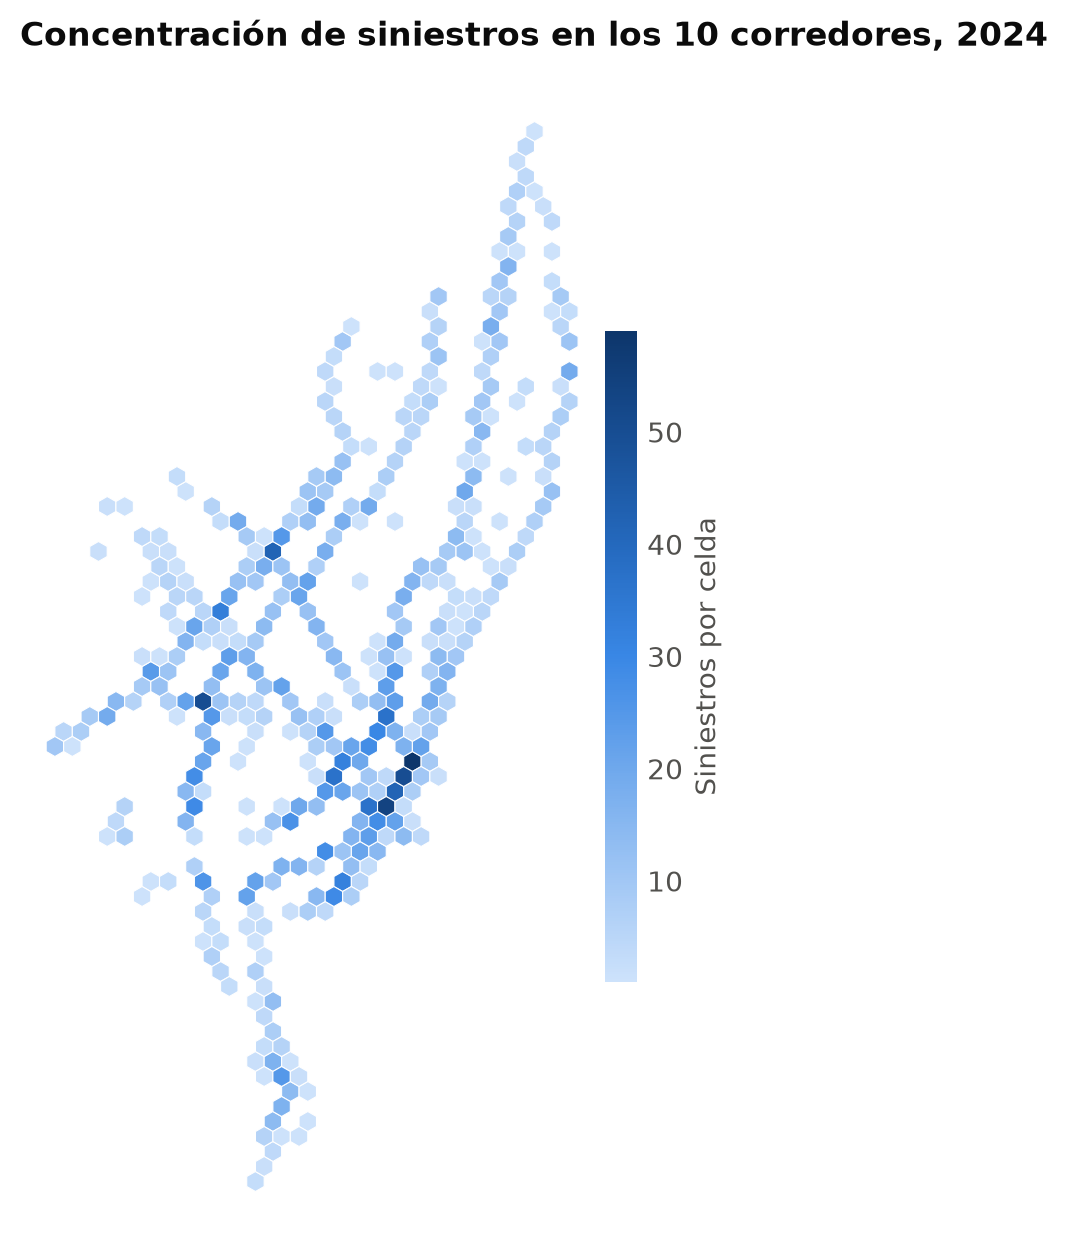
\includegraphics[width=0.78\linewidth,height=0.50\textheight,keepaspectratio]{figuras/oe2_mapa_concentracion.png}
\caption{Mapa de concentración por celdas hexagonales de los siniestros de los corredores seleccionados. El recorte visual de coordenadas no modifica la base de análisis. Fuente: elaboración propia.}
\label{fig:oe2-mapa}
\end{minipage}
\end{figure}

\subsubsection{5.2. Distribución por mes, día y hora}

El mayor conteo mensual se observó en marzo, con 333 siniestros
(9,19\,\%), seguido de agosto, con 330 (9,11\,\%), y septiembre, con
328 (9,05\,\%). Junio y noviembre presentaron los menores valores,
con 253 eventos cada uno (6,98\,\%). La figura \ref{fig:oe2-meses}
permite observar estas variaciones a lo largo del año. Son conteos
mensuales sin ajuste por número de días o volumen de circulación; con
un solo año no se establece un patrón estacional persistente ni se
atribuye la variación a vacaciones, clima u otros factores no medidos.

% Bloque indivisible: la imagen y su pie pasan juntos a la página siguiente.
\begin{figure}[H]
\begin{minipage}{\linewidth}
\centering
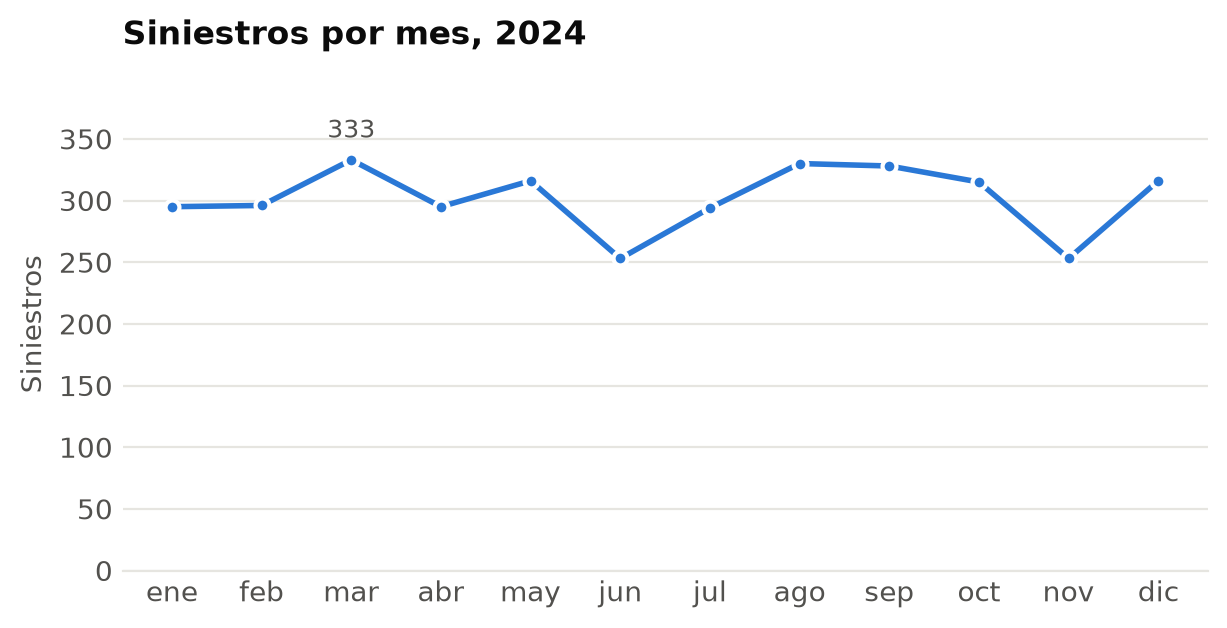
\includegraphics[width=\linewidth,height=0.40\textheight,keepaspectratio]{figuras/oe2_meses.png}
\caption{Distribución mensual de los 3.624 siniestros de 2024. Fuente: elaboración propia con la base depurada.}
\label{fig:oe2-meses}
\end{minipage}
\end{figure}

Por día de la semana, martes registró 571 eventos (15,76\,\%), sábado
570 (15,73\,\%) y viernes 543 (14,98\,\%). Les siguieron jueves
con 530, miércoles con 512 y lunes con 478; domingo presentó el menor
conteo, 420 (11,59\,\%). La diferencia de un evento entre martes y
sábado no permite sostener una superioridad relevante de uno sobre el
otro. Además, los totales no se ajustaron por el número de ocurrencias
de cada día en el calendario de 2024 ni por exposición al tránsito.

El cruce de día y hora (figura \ref{fig:oe2-dia-hora}) permite observar
que el patrón horario no es idéntico todos los días. La celda con mayor
conteo fue martes de 07:00 a 07:59, con 47 eventos durante el año;
también destacaron sábado de 20:00 a 20:59, con 43, y martes de 18:00 a
18:59, con 42. Estos conteos corresponden a combinaciones semanales
acumuladas, no a eventos ocurridos en una sola fecha.

% Bloque indivisible: la imagen y su pie pasan juntos a la página siguiente.
\begin{figure}[H]
\begin{minipage}{\linewidth}
\centering
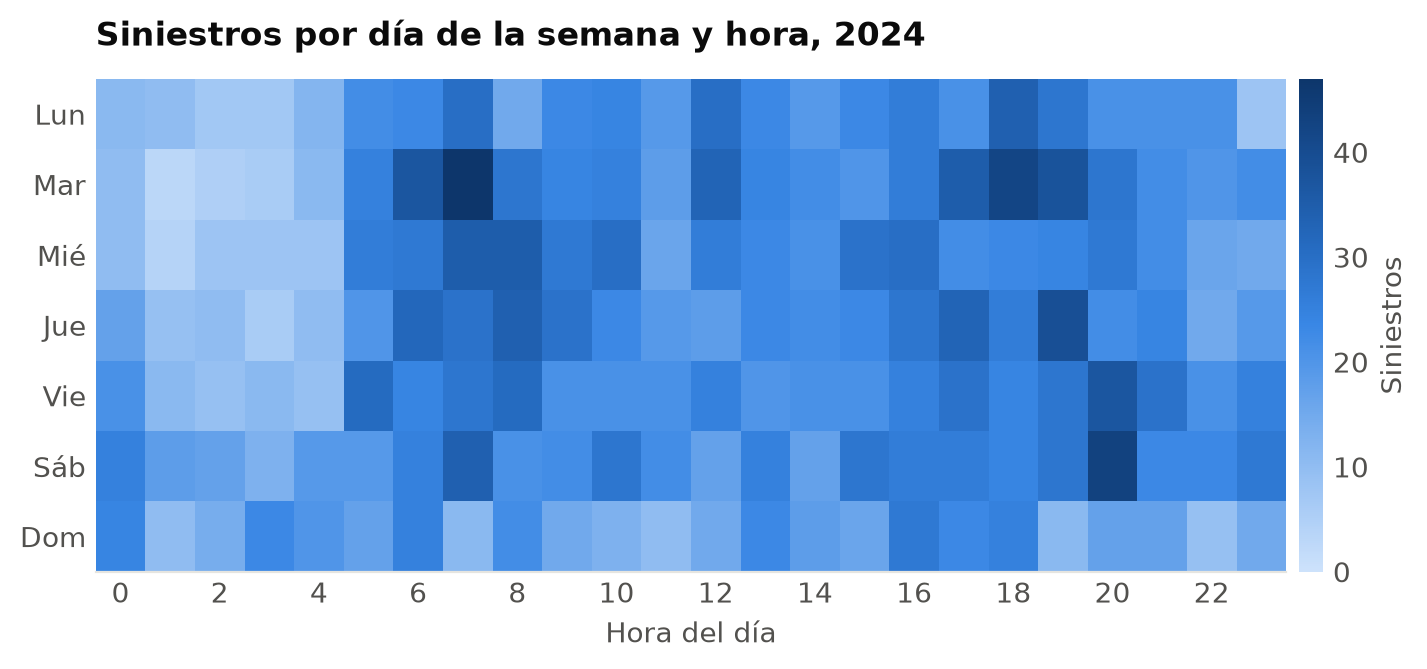
\includegraphics[width=\linewidth,height=0.40\textheight,keepaspectratio]{figuras/oe2_dia_por_hora.png}
\caption{Matriz de siniestros por día de la semana y hora de ocurrencia, acumulados en 2024. Fuente: elaboración propia.}
\label{fig:oe2-dia-hora}
\end{minipage}
\end{figure}

\subsubsection{5.3. Franjas horarias y composición de gravedad}

\begingroup
\begin{longtable}{@{}L{0.25}C{0.18}R{0.18}R{0.16}R{0.23}@{}}
\caption{Frecuencias por franja y ajuste por duración del intervalo.}\label{tab:franjas-oe2}\\
\toprule
\textbf{Franja} & \textbf{Horario} & \textbf{Eventos} & \textbf{\%} & \textbf{Por hora}\\
\midrule
\endfirsthead
\toprule
\textbf{Franja} & \textbf{Horario} & \textbf{Eventos} & \textbf{\%} & \textbf{Por hora}\\
\midrule
\endhead
Madrugada & 00--06 & 576 & 15,89 & 96,00\\
Mañana & 06--10 & 754 & 20,81 & 188,50\\
Mediodía & 10--16 & 914 & 25,22 & 152,33\\
Tarde & 16--20 & 771 & 21,27 & 192,75\\
Noche & 20--24 & 609 & 16,80 & 152,25\\
\bottomrule
\end{longtable}
\endgroup

Las tres franjas con más eventos fueron mediodía, tarde y mañana:
reunieron 2.439 siniestros, equivalentes al 67,30\,\% del total.
Sin embargo, mediodía comprende seis horas y mañana y tarde cuatro;
por eso se complementó el conteo con el cociente entre eventos y ancho
del intervalo. Con ese ajuste, el orden fue tarde (192,75), mañana
(188,50) y mediodía (152,33), apenas por encima de noche (152,25).
El indicador representa eventos acumulados durante el año por cada hora
de anchura de la franja; no significa que ocurran 192,75 siniestros en
una hora de un día particular. La figura \ref{fig:oe2-franjas} presenta
esta comparación.

% Bloque indivisible: la imagen y su pie pasan juntos a la página siguiente.
\begin{figure}[H]
\begin{minipage}{\linewidth}
\centering
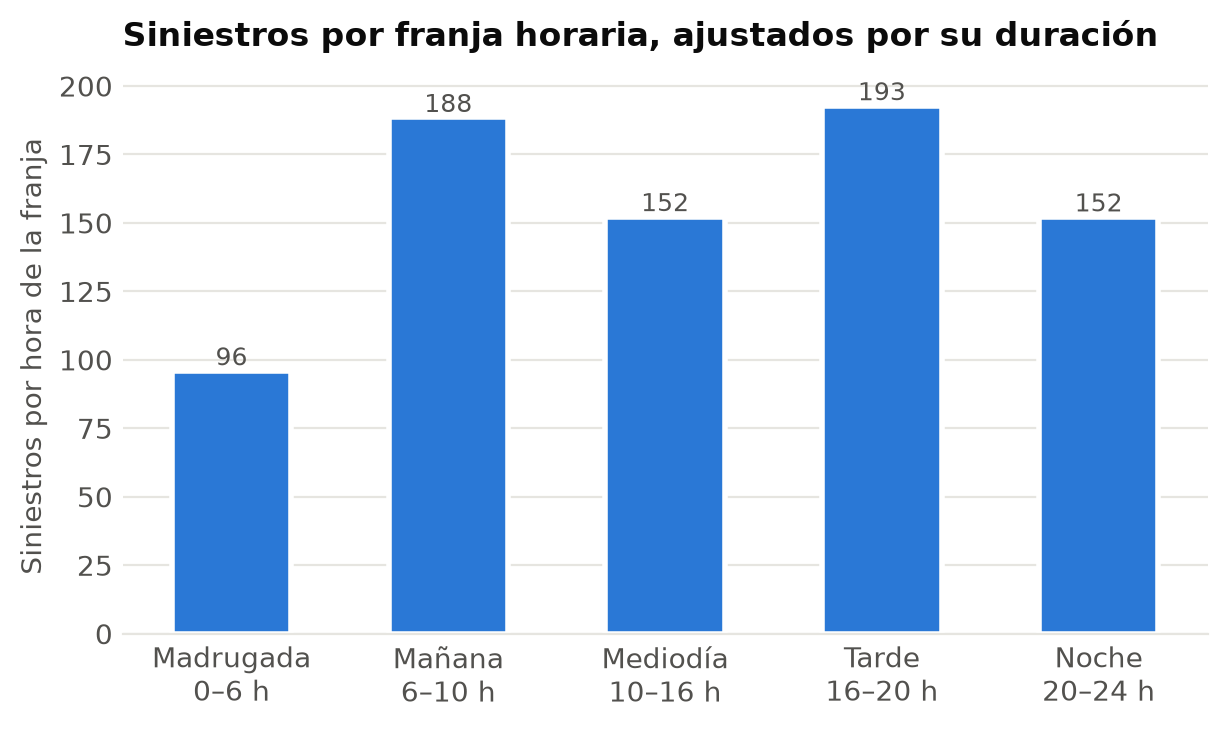
\includegraphics[width=\linewidth,height=0.40\textheight,keepaspectratio]{figuras/oe2_franjas.png}
\caption{Comparación de franjas ajustada por su duración. Las etiquetas del gráfico están redondeadas a enteros; la tabla conserva dos decimales. Fuente: elaboración propia.}
\label{fig:oe2-franjas}
\end{minipage}
\end{figure}

En la base completa, 3.149 eventos se clasificaron con heridos
(86,89\,\%), 279 con solo daños (7,70\,\%) y 196 con muertos
(5,41\,\%). Estas cantidades cuentan siniestros, no personas heridas
o fallecidas. La composición por franja (figura
\ref{fig:oe2-gravedad}) mostró un 7,47\,\% de eventos con muertos
en madrugada y un 6,57\,\% en noche, frente al 4,24\,\% en mañana,
4,92\,\% en mediodía y 4,67\,\% en tarde. Por tanto, las franjas de
mayor volumen no coincidieron con las de mayor proporción de eventos
fatales. Esta comparación es descriptiva; su significancia estadística
corresponde al tercer objetivo.

% Bloque indivisible: la imagen y su pie pasan juntos a la página siguiente.
\begin{figure}[H]
\begin{minipage}{\linewidth}
\centering
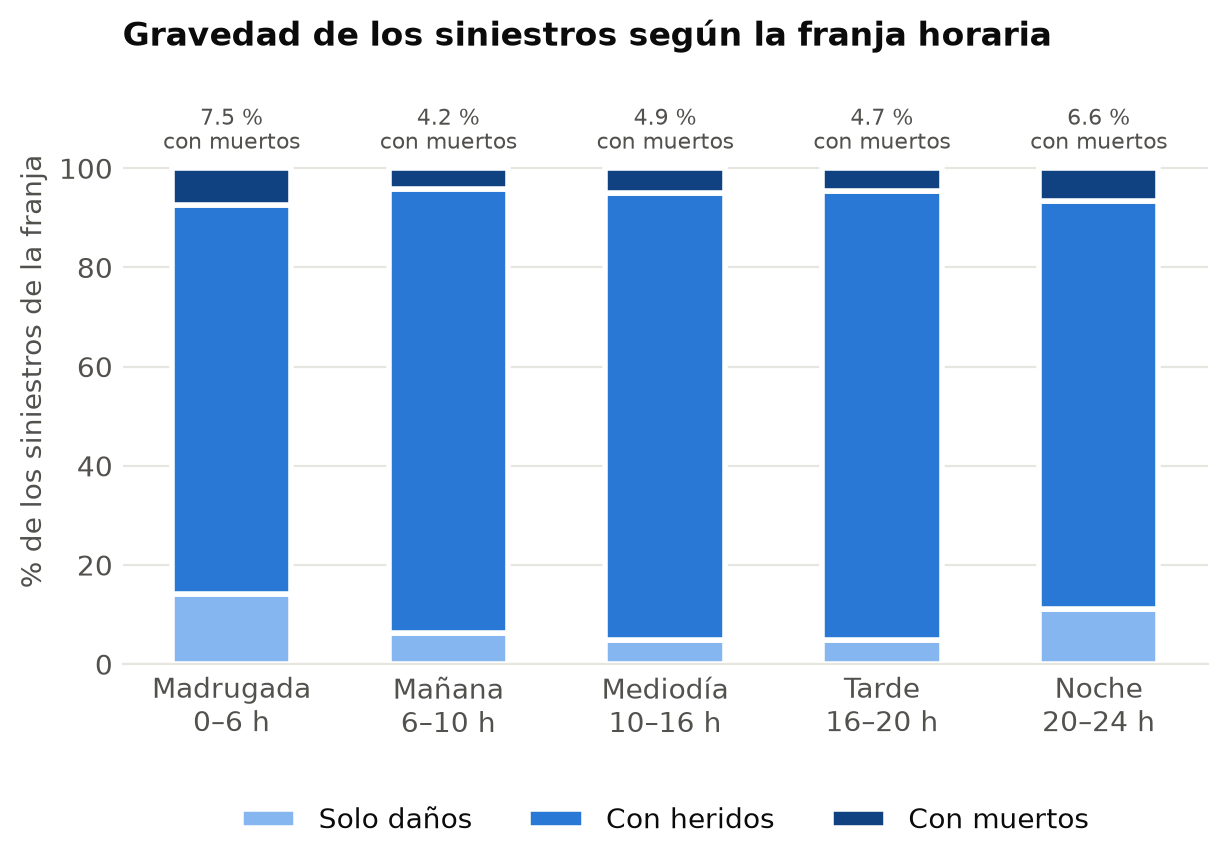
\includegraphics[width=\linewidth,height=0.40\textheight,keepaspectratio]{figuras/oe2_gravedad_por_franja.png}
\caption{Composición porcentual de la gravedad dentro de cada franja horaria. Fuente: elaboración propia.}
\label{fig:oe2-gravedad}
\end{minipage}
\end{figure}

\subsubsection{5.4. Participación de actores y clases de siniestro}

La motocicleta apareció marcada en 2.330 siniestros (64,29\,\%), el
peatón en 675 (18,63\,\%) y el transporte público de pasajeros en
667 (18,41\,\%). También se registraron personas mayores en 650
(17,94\,\%), bicicletas en 443 (12,22\,\%), taxi u otro transporte
público individual en 376 (10,38\,\%), vehículos de carga en 306
(8,44\,\%) y menores de edad en 218 (6,02\,\%). La figura
\ref{fig:oe2-actores} reúne estos indicadores. Las categorías combinan
tipos de vehículo y grupos de personas, y no son excluyentes: un mismo
evento puede involucrar motocicleta, peatón y persona mayor. En
consecuencia, sus porcentajes no suman 100\,\% ni constituyen un
recuento de víctimas por actor.

% Bloque indivisible: la imagen y su pie pasan juntos a la página siguiente.
\begin{figure}[H]
\begin{minipage}{\linewidth}
\centering
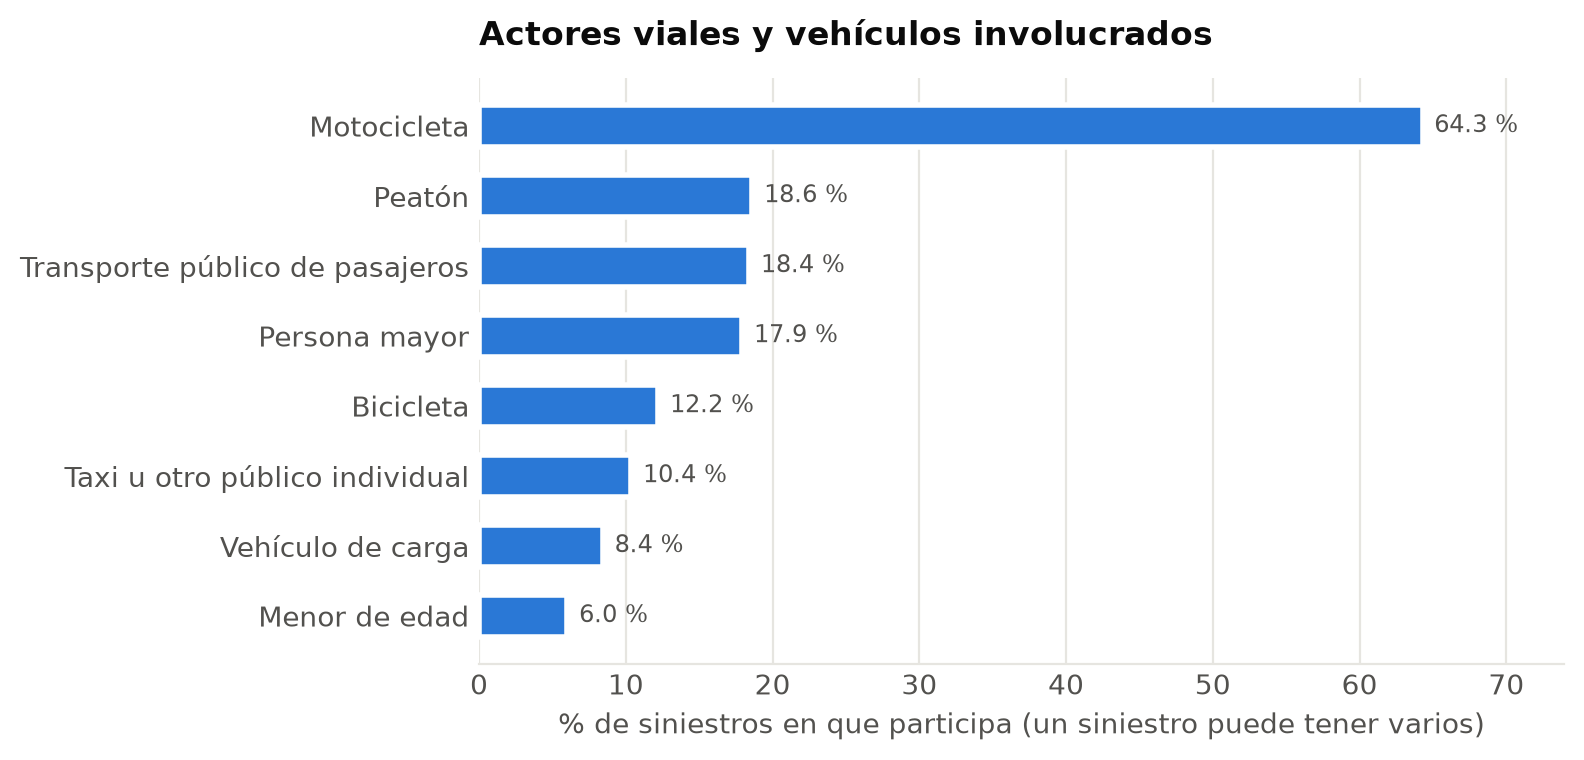
\includegraphics[width=\linewidth,height=0.40\textheight,keepaspectratio]{figuras/oe2_actores.png}
\caption{Participación registrada de actores y vehículos en los siniestros. Las categorías pueden coincidir en un mismo evento. Fuente: elaboración propia.}
\label{fig:oe2-actores}
\end{minipage}
\end{figure}

Por clase, predominaron los choques, con 2.583 eventos (71,27\,\%),
seguidos de atropellos, con 652 (17,99\,\%), caídas de ocupante,
con 204 (5,63\,\%), y volcamientos, con 133 (3,67\,\%). Se
registraron además 50 eventos clasificados como otro (1,38\,\%) y dos
incendios (0,06\,\%). La presencia de peatón y la clase atropello no
son variables equivalentes: una describe la participación registrada y
la otra la modalidad del evento, por lo que sus conteos no tienen que
coincidir.

\subsubsection{5.5. Síntesis del cumplimiento de los dos objetivos}

El primer objetivo produjo una base de 3.624 eventos únicos de 2024,
con 77 columnas, diccionario operativo, corredores y longitudes,
trazabilidad y menos del 5\,\% de nulos en las variables clave. Su
lectura conserva las limitaciones de la codificación de indicadores,
la asignación de intersecciones y la validación geográfica por ventana.

El segundo objetivo produjo nueve tablas descriptivas, seis gráficos y
los mapas de concentración estático e interactivo. Se identificaron
Boyacá, Caracas y NQS como los tres corredores de mayor conteo, y
Carrera 10, NQS y Calle 6 como los de mayor concentración por kilómetro.
Las franjas de mayor conteo fueron mediodía, tarde y mañana; al ajustar
por duración, tarde y mañana ocuparon los primeros lugares. La alta
participación registrada de motocicleta y la diferencia entre volumen
y composición de gravedad aportan una caracterización para los análisis
posteriores, sin anticipar sus pruebas o conclusiones.

\clearpage
\section{Referencias bibliográficas}

\begin{enumerate}
\tightlist
\item
  Chand, A., Jayesh, S., \& Bhasi, A. B. (2021). Road traffic accidents:
  An overview of data sources, analysis techniques and contributing
  factors. Materials Today: Proceedings, 47, 5135--5141.
  \url{https://doi.org/10.1016/j.matpr.2021.05.415}
\item
  Sathiyanathan, R., \& Warnajith, N. (2024). Integration of k-means
  clustering and association rule mining for road safety analysis. In
  2024 International Conference on Smart Computing and Systems
  Engineering (SCSE) (pp.~1--7). IEEE.
  \url{https://doi.org/10.1109/SCSE61872.2024.10550547}
\item
  Shahin, M., et al.~(2021). Cluster-based association rule mining for
  an intersection accident dataset. In 2021 International Conference on
  Computing, Electronic and Electrical Engineering (ICE Cube)
  (pp.~1--6). IEEE.
  \url{https://doi.org/10.1109/ICECube53880.2021.9628206}
\item
  Job, R. F. S. (2022). Evaluations of speed camera interventions can
  deliver a wide range of outcomes: Causes and policy implications.
  Sustainability, 14(3), Article 1765.
  \url{https://doi.org/10.3390/su14031765}
\item
  Klaylee, J., Iamtrakul, P., \& Sornlertlamvanich, V. (2022).
  Identification of suburban motorcycle traffic accident hotspots using
  GIS-based spatial analysis. In 2022 10th International Conference on
  Traffic and Logistic Engineering (ICTLE) (pp.~35--40). IEEE.
  \url{https://doi.org/10.1109/ICTLE55577.2022.9902103}
\item
  Ospina-Mateus, H., Berrio García, S., Quintana Jiménez, L., \&
  Salas-Navarro, K. (2022). Dataset of traffic accidents in
  motorcyclists in Bogotá, Colombia. Data in Brief, 43, Article 108461.
  \url{https://doi.org/10.1016/j.dib.2022.108461}
\item
  Vargas Montero, F. (2022). Análisis de datos de accidentalidad vial de
  la ciudad de Bogotá a partir de datos abiertos y datos obtenidos desde
  redes sociales {[}Trabajo de grado, Universidad Nacional de
  Colombia{]}. \url{https://repositorio.unal.edu.co/handle/unal/81571}
\item
  Bejar Gladkowski, A. A. (2023). Análisis predictivo de accidentes de
  tráfico en la ciudad de Madrid {[}Trabajo de fin de grado, Universitat
  Oberta de Catalunya{]}.
  \url{https://openaccess.uoc.edu/handle/10609/147306}
\item
  Zhang, Y., Zhu, F., Li, Q., Qiu, Z., \& Xie, Y. (2023). Exploring
  spatiotemporal patterns of expressway traffic accidents based on
  density clustering and Bayesian network. ISPRS International Journal
  of Geo-Information, 12(2), Article 73.
  \url{https://doi.org/10.3390/ijgi12020073}
\item
  Ordoñez Cueto, J. L., \& Fernández Ebratt, L. V. (2025). Diseño de un
  dashboard para el análisis de los datos relacionados con los
  accidentes ocurridos en la ciudad de Barranquilla {[}Trabajo de grado,
  Universidad Nacional Abierta y a Distancia{]}.
  \url{https://repository.unad.edu.co/handle/10596/67670}
\end{enumerate}

\end{document}
